\chapter{BÁO CÁO KỸ THUẬT}\label{chap:kythuat}

Mã nguồn gồm 8 gói Python, trong đó 7 gói chạy độc lập bằng \code{python -m scholarlens.<module>} và cùng dùng
chung thư mục \code{data/}. Phần nặng (embedding hàng loạt, chạy LLM) chạy trên máy GPU; máy demo chỉ cần CPU để
chạy web app và embedding từng PDF mới.

\section{Cấu trúc mã nguồn và các module}

\begin{table}[H]
\centering\small\setstretch{1.15}
\begin{tabularx}{\linewidth}{@{}P{0.15\linewidth}P{0.3\linewidth}L@{}}
\toprule
\textbf{Module} & \textbf{Tệp chính} & \textbf{Lệnh chạy độc lập (ví dụ)}\\
\midrule
\code{crawler} & \code{arxiv\_client.py} & \code{crawler keyword}, \code{crawler category}, \code{crawler ids}, \code{crawler snapshot}\\
\code{ingest} & \code{pdf\_parser.py}, \code{chunker.py}, \code{pipeline.py} & \code{ingest jsonl}, \code{ingest pdf}, \code{ingest dir}, \code{ingest all}\\
\code{embedding} & \code{embedder.py}, \code{pipeline.py} & \code{embedding --device cuda}, \code{embedding --rebuild}\\
\code{graph} & \code{knowledge\_graph.py}, \code{keywords.py}, \code{builder.py} & \code{graph build}, \code{graph stats}, \code{graph related <mã bài>}\\
\code{retrieval} & \code{hybrid.py}, \code{graph\_rag.py} & Dùng qua chatbot và web app\\
\code{chat} & \code{llm.py}, \code{prompts.py}, \code{chatbot.py} & \code{chat --mode research}\\
\code{llm\_server} & \code{server.py} & \code{llm\_server --preset qwen2.5-7b-awq --tunnel cloudflared}\\
\code{app} & \code{server.py}, \code{static/} & \code{app --port 7860}\\
\bottomrule
\end{tabularx}
\caption{Các module của ScholarLens}\label{tab:module}
\end{table}

\section{Triển khai}

\begin{enumerate}[label=(\arabic*)]
\item \textbf{Trên máy GPU (Kaggle, 2 GPU T4):} mã nguồn và dữ liệu được đóng gói thành Kaggle Dataset
  (\code{scripts/make\_kaggle\_bundle.py}). Notebook \code{kaggle\_llm\_server.ipynb} lần lượt embedding và dựng
  đồ thị, đóng gói thư mục \code{data/} để tải về, cài vLLM, chạy mô hình, mở tunnel và giữ phiên sống.
\item \textbf{Trên máy demo:} giải nén thư mục \code{data/}, chạy \code{python -m scholarlens.app} hoặc
  \code{docker compose up -d --build}, mở trình duyệt và dán URL tunnel cùng API key vào dòng ``LLM''.
\end{enumerate}

Image Docker dùng \code{python:3.11-slim} với torch bản CPU và đã tải sẵn model embedding, nên chạy được mà không
cần mạng để tải model; thư mục \code{data/} được gắn vào container nên dữ liệu không mất khi xóa container. Máy GPU
và máy demo phải dùng cùng model embedding, vì vector câu hỏi và vector trong kho phải nằm trong cùng không gian.

\section{Giao diện}

Giao diện được giữ tối giản (Hình~\ref{fig:giaodien}). Thanh bên thu gọn hoặc mở rộng được, chứa lịch sử hội thoại
và dòng kết nối LLM. Khung chat hiển thị câu trả lời dần từng chữ; dưới mỗi câu trả lời có danh sách nguồn thu gọn
và nút xem đồ thị của câu trả lời đó. Đồ thị mở được toàn màn hình (Hình~\ref{fig:dothi}); bấm vào từng nút để xem
chi tiết. PDF được thêm bằng nút đính kèm hoặc kéo-thả vào cửa sổ.

\begin{figure}[H]
\centering
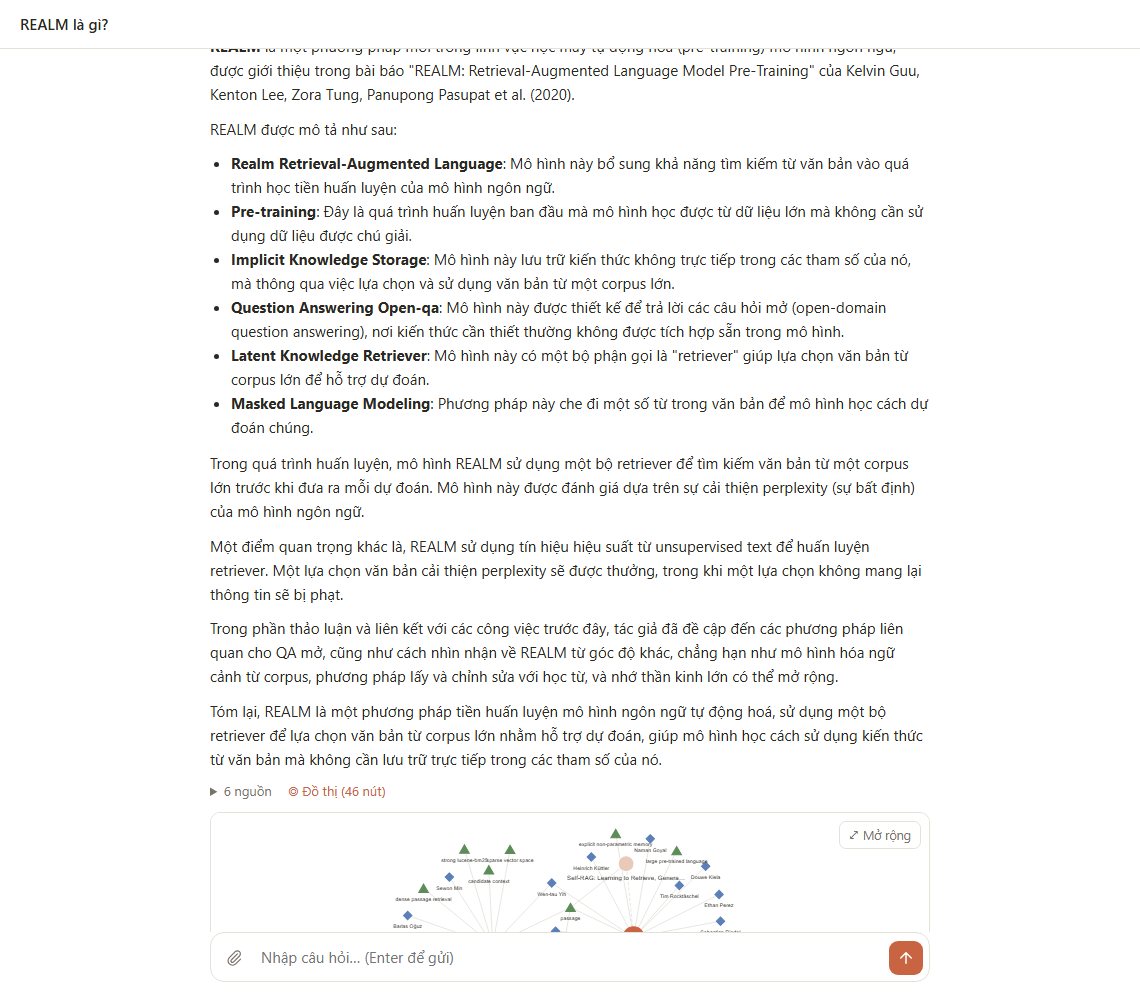
\includegraphics[width=0.85\linewidth]{figures/app_chat.png}
\caption{Khung chat: câu trả lời tiếng Việt có trích dẫn, danh sách nguồn và đồ thị của câu trả lời}\label{fig:giaodien}
\end{figure}

\begin{figure}[H]
\centering
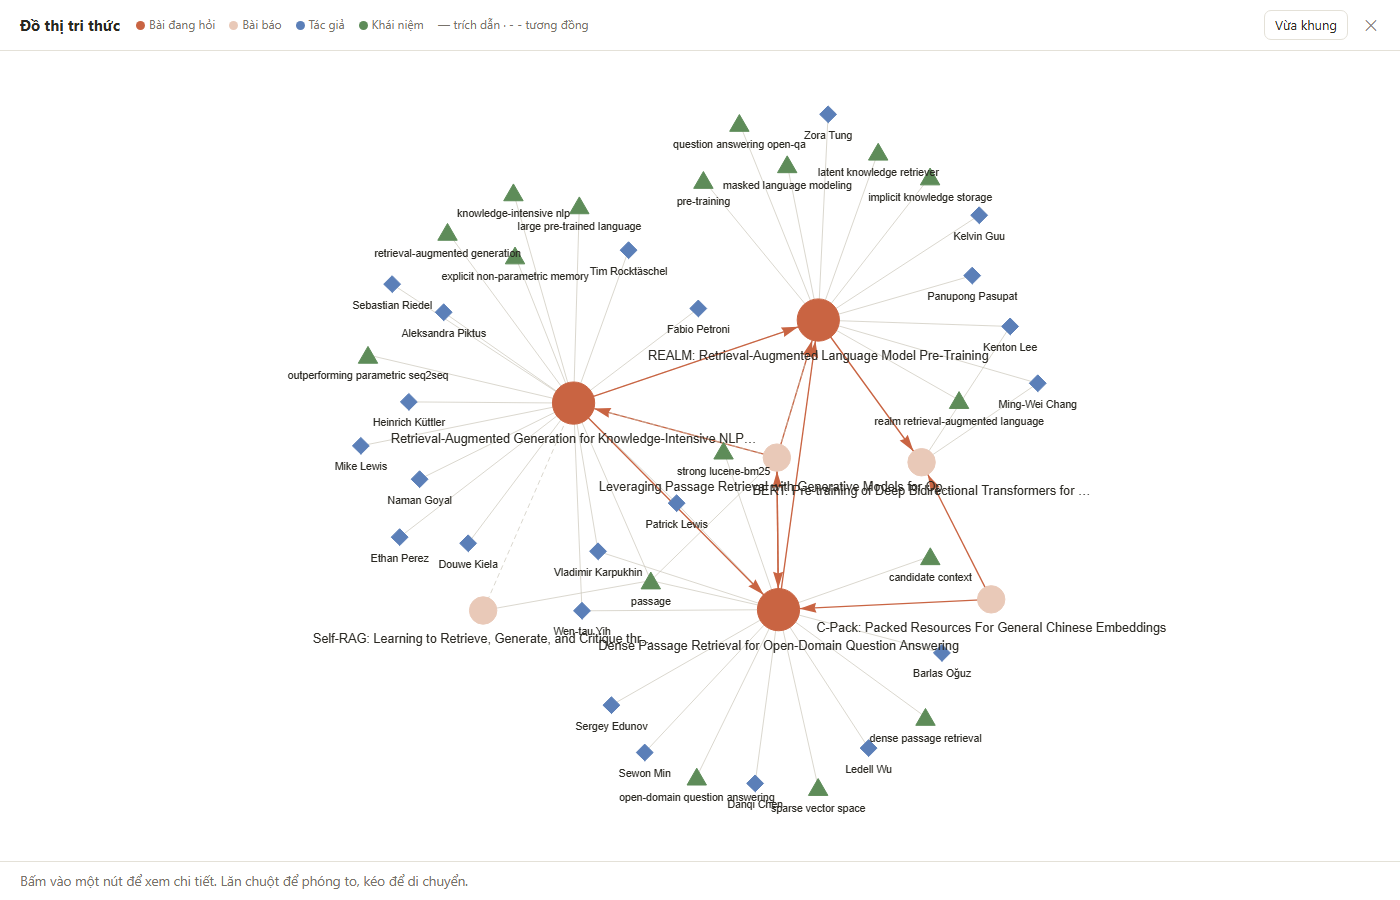
\includegraphics[width=\linewidth]{figures/app_graph_full.png}
\caption{Đồ thị toàn màn hình: bài đang hỏi (cam đậm), bài liên quan, tác giả, khái niệm và các cạnh trích dẫn}\label{fig:dothi}
\end{figure}

\section{Đánh giá}\label{sec:danhgia}

Script \code{scripts/evaluate.py} đo ba khía cạnh trên kho 492 bài:
\begin{itemize}
\item \textbf{Tìm bài theo tiêu đề (known-item):} truy vấn là tiêu đề, kho tìm kiếm là các tóm tắt không chứa tiêu
  đề, đáp án duy nhất là chính bài đó. Độ đo Recall@$k$ (tỉ lệ câu hỏi có đáp án nằm trong $k$ kết quả đầu) và
  MRR@10 (trung bình của $1/\text{hạng}$ của đáp án).
\item \textbf{Kiểm tra trùng:} 200 tiêu đề bị biến đổi ngẫu nhiên (chữ thường, bỏ dấu câu, bỏ một từ, thêm
  ``(Extended Version)''), cộng kiểm tra báo nhầm trên toàn bộ 492 tiêu đề thật.
\item \textbf{Đồ thị:} tỉ lệ bài liên quan (top-5) cùng chuyên mục chính với bài gốc, so với chọn ngẫu nhiên.
\end{itemize}

\begin{table}[H]
\centering\small\setstretch{1.15}
\begin{tabularx}{\linewidth}{@{}Lccccl@{}}
\toprule
\textbf{Phương pháp} & \textbf{R@1} & \textbf{R@5} & \textbf{R@10} & \textbf{MRR@10} & \textbf{Ghi chú}\\
\midrule
BM25 & 0,957 & 0,992 & 0,996 & 0,973 & 1,4 ms / truy vấn\\
Dense (multilingual-e5-base) & --- & --- & --- & --- & chưa chạy\\
Dense (bge-base-en-v1.5) & --- & --- & --- & --- & chưa chạy\\
Hybrid RRF (e5 + BM25) & --- & --- & --- & --- & chưa chạy\\
\bottomrule
\end{tabularx}
\caption{Kết quả tìm bài theo tiêu đề}\label{tab:knownitem}
\end{table}

BM25 đạt điểm rất cao vì từ của tiêu đề gần như luôn xuất hiện lại trong tóm tắt, nên bài kiểm tra này chủ yếu
xác nhận pipeline hoạt động đúng. Các dòng dense và hybrid cần chạy lại script trên GPU. Lợi ích của embedding thể
hiện rõ hơn ở câu hỏi tiếng Việt: trong kiểm thử chức năng, truy vấn ``phương pháp truy xuất dựa trên đồ thị cho
RAG'' đưa LightRAG lên hạng 1 dù chỉ có từ ``RAG'' trùng với văn bản tiếng Anh.

\begin{table}[H]
\centering\small\setstretch{1.15}
\begin{tabularx}{\linewidth}{@{}Lr@{}}
\toprule
\textbf{Kiểm tra trùng} & \textbf{Kết quả}\\
\midrule
Phát hiện theo mã arXiv & 100\% (200/200)\\
Phát hiện tiêu đề bị biến đổi & 95\% (190/200)\\
Báo nhầm trên 492 tiêu đề thật & 0\%\\
Báo nhầm với tiêu đề đối kháng (``<tiêu đề A> for X Revisited'') & 19\%\\
\bottomrule
\end{tabularx}
\caption{Kết quả kiểm tra trùng}\label{tab:dedup}
\end{table}

\begin{table}[H]
\centering\small\setstretch{1.15}
\begin{tabularx}{\linewidth}{@{}P{0.38\linewidth}L@{}}
\toprule
\textbf{Đồ thị tri thức} & \textbf{Kết quả}\\
\midrule
Quy mô & 5.598 nút (492 bài, 2.232 tác giả, 2.805 khái niệm, 69 chuyên mục), 8.258 cạnh\\
Cạnh theo loại & MENTIONS 2.952; WRITTEN\_BY 2.354; SIMILAR\_TO 2.052; IN\_CATEGORY 881; CITES 19\\
Bài có ít nhất một bài liên quan & 100\%\\
Bài liên quan (top-5) cùng chuyên mục & 37\% (chọn ngẫu nhiên: 14\%, tức gấp 2,7 lần)\\
\bottomrule
\end{tabularx}
\caption{Kết quả đánh giá đồ thị}\label{tab:graph}
\end{table}

Số cạnh CITES còn ít (19) vì chỉ 12 bài có toàn văn PDF; bài chỉ có metadata thì không có danh sách tài liệu
tham khảo.

\section{Kiểm thử chức năng}

\begin{table}[H]
\centering\small\setstretch{1.15}
\begin{tabularx}{\linewidth}{@{}P{0.4\linewidth}L@{}}
\toprule
\textbf{Kịch bản} & \textbf{Kết quả quan sát}\\
\midrule
Thêm PDF LightRAG (16 trang) & Tra arXiv API, 38 đoạn, 5 cạnh tương đồng, 6 khái niệm; khoảng 32 giây trên CPU\\
Thêm lại cùng file & Báo ``trùng nội dung file (SHA-256)'' ngay lập tức\\
Thêm PDF đã có từ bước thu thập (RAG, 2005.11401) & Báo ``trùng mã arXiv'' sau 0,2 giây\\
Tải lên hàng loạt 2 PDF qua web & Mỗi file một trạng thái riêng: 1 mới (6 bước), 1 trùng\\
Hỏi ``Tóm tắt bài này'' khi có bài focus & Chế độ Research, 5 nguồn, đồ thị con 17 nút\\
``xin chào'' & Định tuyến sang chế độ Chat\\
GraphRAG và LightRAG cùng trong kho & Tự sinh cạnh ``LightRAG trích dẫn GraphRAG'' từ References\\
Tunnel trycloudflare chết giữa chừng & \code{keep\_alive} tự mở tunnel mới; ứng dụng trả lời bằng chế độ trích đoạn trong lúc mất kết nối\\
\bottomrule
\end{tabularx}
\caption{Kết quả kiểm thử chức năng}\label{tab:kiemthu}
\end{table}

\section{Hạn chế}

\begin{itemize}
\item \textbf{Đọc PDF bằng quy tắc:} bảng, công thức và bố cục hai cột phức tạp có thể lộn thứ tự; tác giả trích
  từ PDF kém tin cậy khi không tra được arXiv API.
\item \textbf{Trích dẫn chỉ qua mã arXiv:} tài liệu tham khảo không ghi mã arXiv (bài hội nghị, tạp chí) chưa trở
  thành cạnh CITES.
\item \textbf{Khái niệm là n-gram:} đôi khi lấy cụm chung chung, làm giảm độ chính xác của cạnh MENTIONS.
\item \textbf{Embedding trên CPU chậm:} khoảng 1,4 đoạn/giây với e5-base, nên mỗi PDF mới mất chừng 30 giây khi
  demo trên máy không có GPU.
\item \textbf{Kiểm tra trùng với tiêu đề đối kháng:} tiêu đề mới chứa nguyên văn tiêu đề cũ cộng vài từ có thể bị
  báo trùng nhầm (19\% trong phép thử đối kháng).
\item \textbf{Ngôn ngữ của Qwen2.5:} mô hình đôi khi chuyển sang tiếng Trung giữa câu trả lời. Hệ thống đã thêm
  quy tắc ngôn ngữ vào prompt và lời nhắc trong từng lượt hỏi tiếng Việt; hiệu quả cần được theo dõi thêm.
\end{itemize}
